\newcommand{\JvolveTimeLine}[5]{
\begin{center}
\begin{tikzpicture}[auto]
  \tikzstyle{block}=[
    font=\tiny,
    rectangle,
    draw=structure.fg,
    thick,
    text width=1.2cm,
    text badly centered,
    rounded corners,
    minimum height=2em,
  ]
  \tikzstyle{current}=[fill=structure.fg!20, ]
  \tikzstyle{line}=[draw, thick, -latex',]
  \tikzstyle{every path}=[line]
  \matrix [column sep=5mm,row sep=7mm,ampersand replacement=\&] {
    \node [block,#1] (0) {\hyperlink{offline}{Offline tool}};          \&
    \node [block,#2] (1) {\hyperlink{suspend}{Suspend application}};   \&
    \node [block,#3] (2) {\hyperlink{classload}{Load new classes}};    \&
    \node [block,#4] (3) {\hyperlink{transform}{Transform objects}};   \&
    \node [block,#5] (4) {Resume application};                         \\
  };
  \path (0) -- (1);
  \path (1) -- (2);
  \path (2) -- (3);
  \path (3) -- (4);
\end{tikzpicture}
\end{center}
}


\subsection{Implementation}
\ShowTOC

\begin{frame}[t,fragile]{Update process}%{A Sub-title is optional}
\JvolveTimeLine{}{}{}{}{}
\begin{itemize}
\item Offline Update Preparation Tool (UPT)
\item \DSU{} VM
  \begin{itemize}
  \item Reach a safe point in the VM%(thread synchronization)
  \item Install new classes%(classloader)
  \item Transform objects to new definition%(garbage collector)
  \item Resume execution
  \end{itemize}
\end{itemize}
\end{frame}

\begin{frame}[t,fragile,label=offline]{Update Preparation Tool}%{A Sub-title is optional}
% \vspace{-2ex}
\JvolveTimeLine{current}{}{}{}{}
% \vspace{-2ex}
\begin{itemize}
\item Uses jclasslib\footnote{\url{http://jclasslib.sourceforge.net}}, a
bytecode library
\item Compares bytecodes of the two versions
% \item Categorizes changes into
%   \begin{description}
%   \item[Updated classes] Classes that add, remove, change signature of fields
%                        or methods
%   \item[Updated methods] Changes within a method body. Only the method has
%                         to be loaded/updated
%   \item[Indirect updates] No change to method, but refers to changed
%                           classes
%   \end{description}
\item Generates old version stubs and default object transformers
\end{itemize}
\end{frame}

\begin{frame}[t,fragile]{Compiling transformation functions}%{A Sub-title is optional}
\begin{itemize}
\item All transformers specified in a separate source file
\item Class transformers  \\ \hspace{6ex} {\footnotesize {\tt jvolveClass(ClassName unused)}}
\item Object transformers \\ \hspace{6ex} {\footnotesize {\tt jvolveObject(old\_ClassName from, ClassName to)}}
\item Compiled specially by a JastAddJ extension to the Java language
\item Ignores access protection and allows assigning to {\tt final} fields
\end{itemize}
\end{frame}

\begin{frame}[t,fragile,label=suspend]{Safe point for the update}%{A Sub-title is optional}
\JvolveTimeLine{}{current}{}{}{}
\begin{itemize}
\item Update must be atomic
\item Updates happen at ``safe points''\\
      (VM yield points with restriction on what methods can be on stack)
\item Extend the thread scheduler to suspend all application threads
\item Examine all stacks, ensure no restricted methods on stack and perform
      the update
\end{itemize}
\end{frame}

\begin{frame}[t,fragile]{Restricted methods}%{A Sub-title is optional}
\begin{enumerate}[(1)]
\item Methods changed by the update
\item Methods whose bytecode is unchanged, but compiled representation is
      changed by the update
  \begin{itemize}
  \item Offsets of fields and methods hard-coded in machine code
  \item Inlined callees may have changed
  \end{itemize}
\item Methods identified by the user as unsafe based on semantic
information about the application
\end{enumerate}
\uncover<2>{
Handling restricted methods
\begin{itemize}
\item \emph{On-stack replace} baseline-compiled category (2) methods
\item Do not allow (1) and (3) to be active on stack, install a return
      barrier for such methods
\end{itemize}
}
\end{frame}

\begin{frame}{Handling restricted methods}%{A Sub-title is optional}
\vspace*{-2mm}%
\begin{center}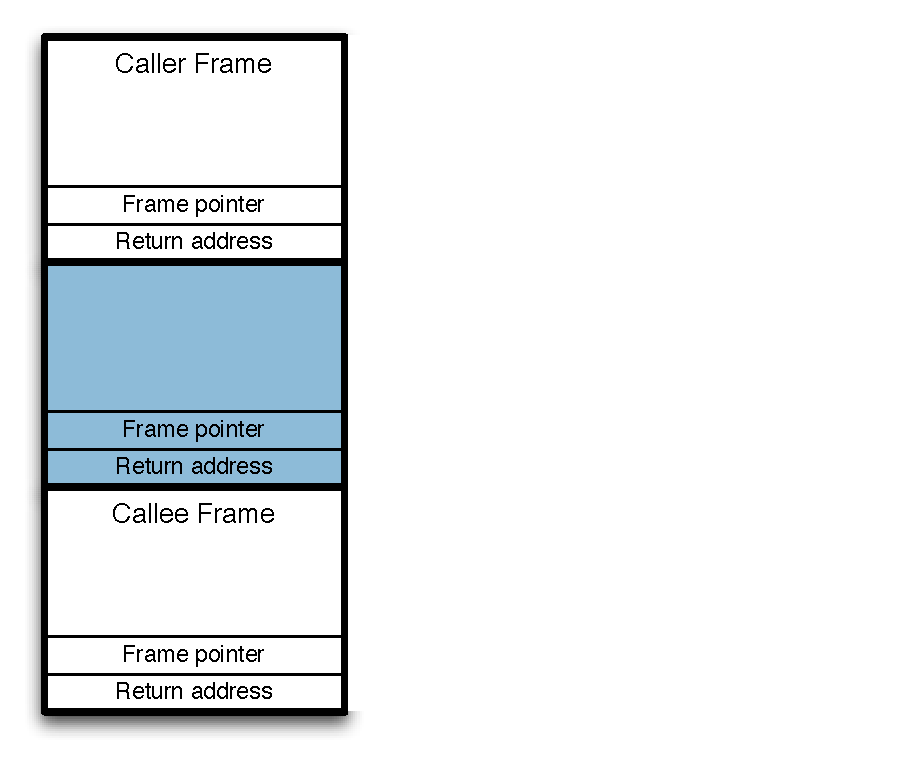
\includegraphics[scale=0.62]{images/stack-smash/stack-frames-overview}\end{center}
\end{frame}

\begin{frame}{Performing On-stack replacement}%{A Sub-title is optional}
\vspace*{-2mm}%
\begin{center}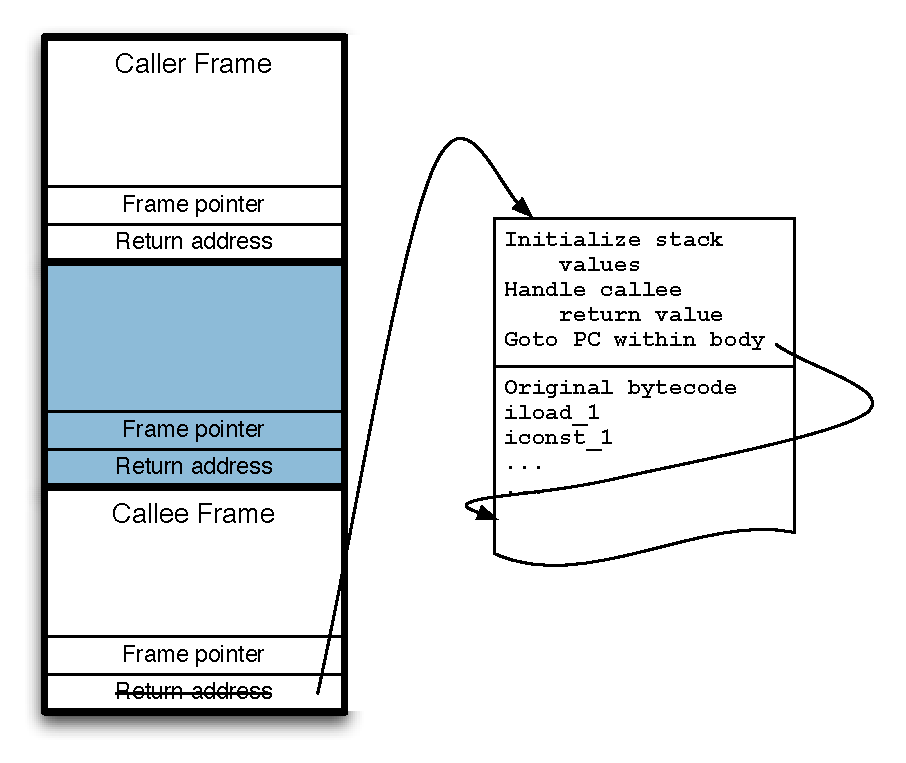
\includegraphics[scale=0.62]{images/stack-smash/osr-overview}\end{center}
\end{frame}

\begin{frame}{Installing return barrier for DSU}%{A Sub-title is optional}
\vspace*{-2mm}%
\begin{center}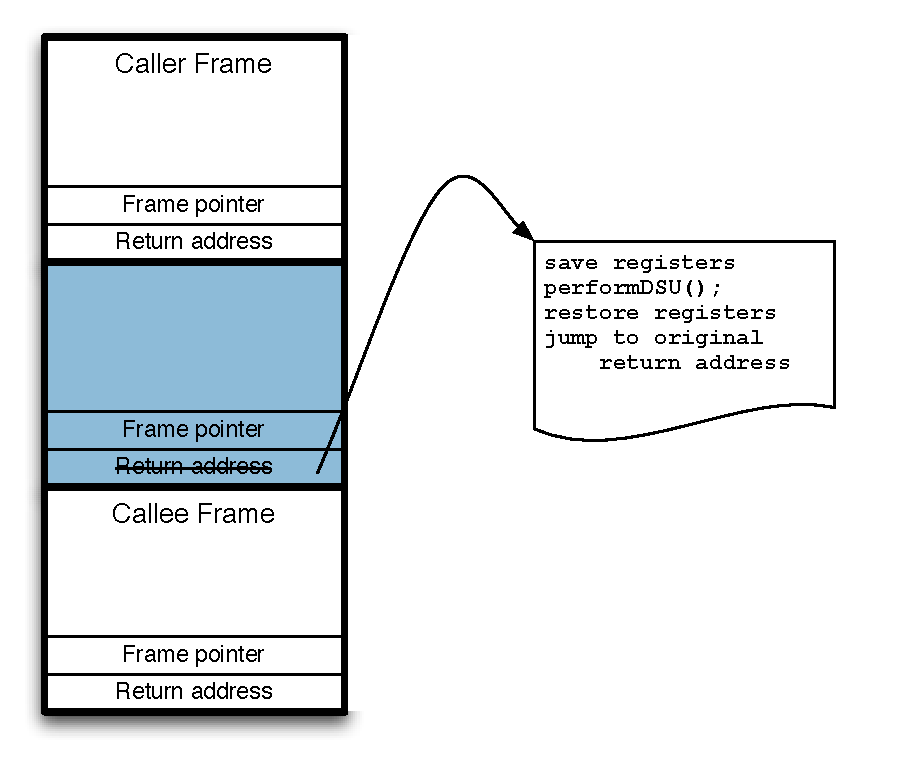
\includegraphics[scale=0.62]{images/stack-smash/return-barrier-overview}\end{center}
\end{frame}

\begin{frame}{Reaching a safe point}%{A Sub-title is optional}
\hspace*{-3mm}
\scalebox{0.44}{%
\uncover<1>{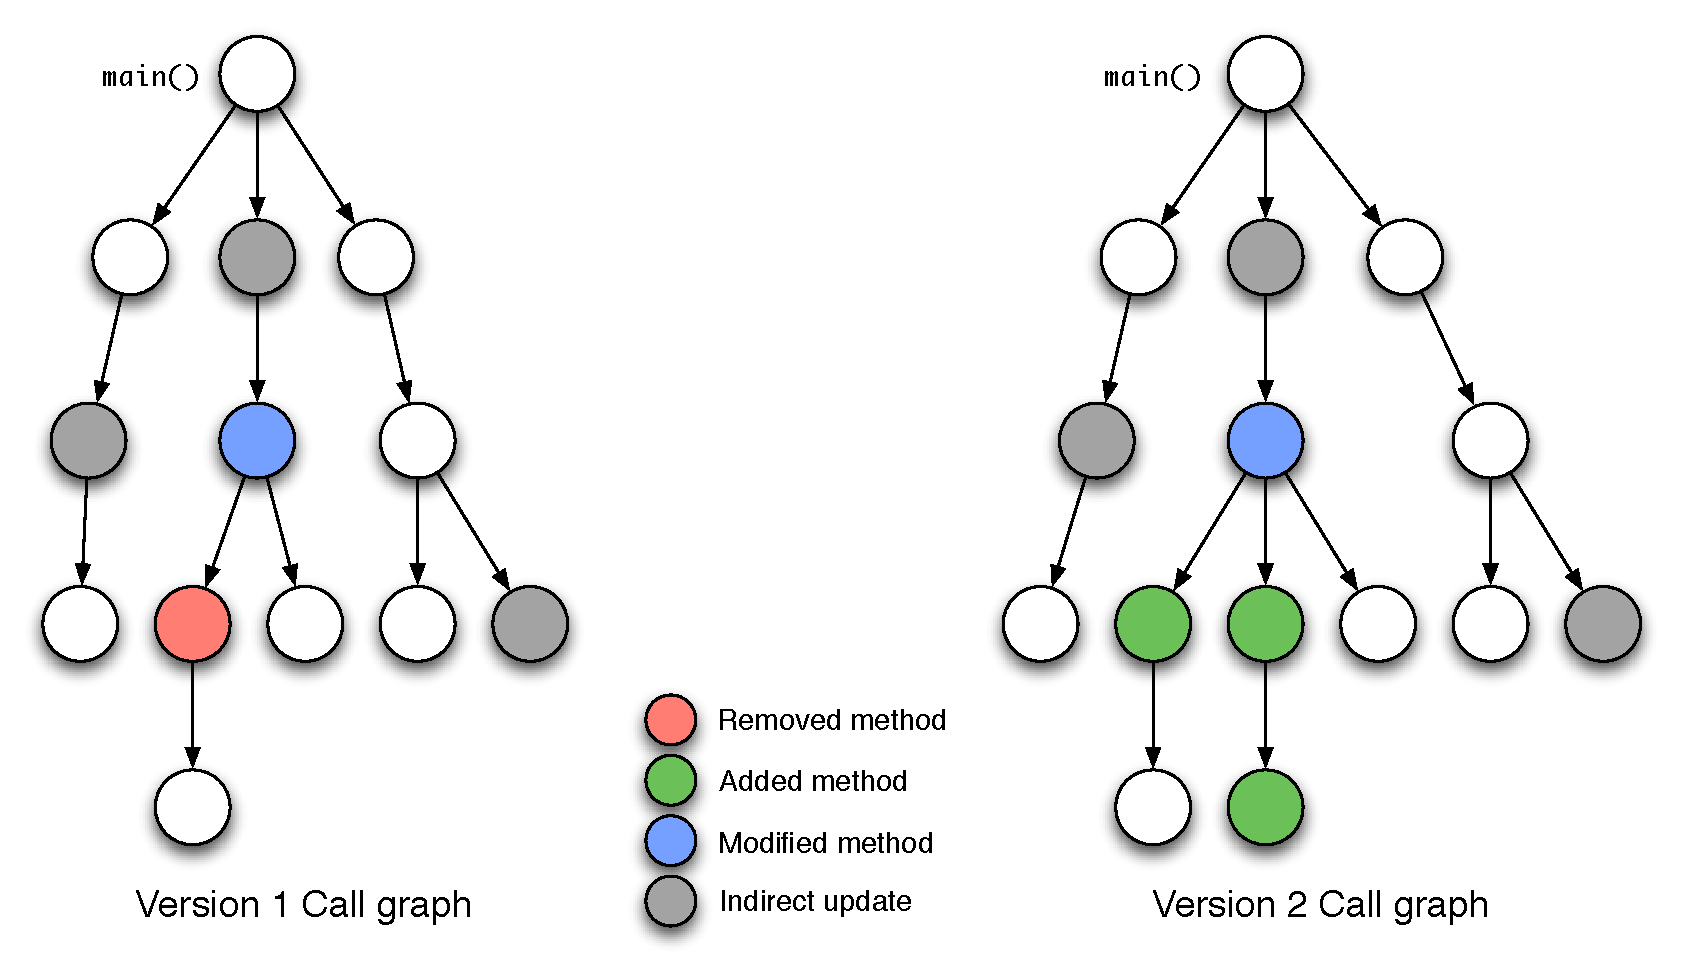
\includegraphics{images/safe-point-call-graph/both-call-graphs-1}}%
\uncover<2>{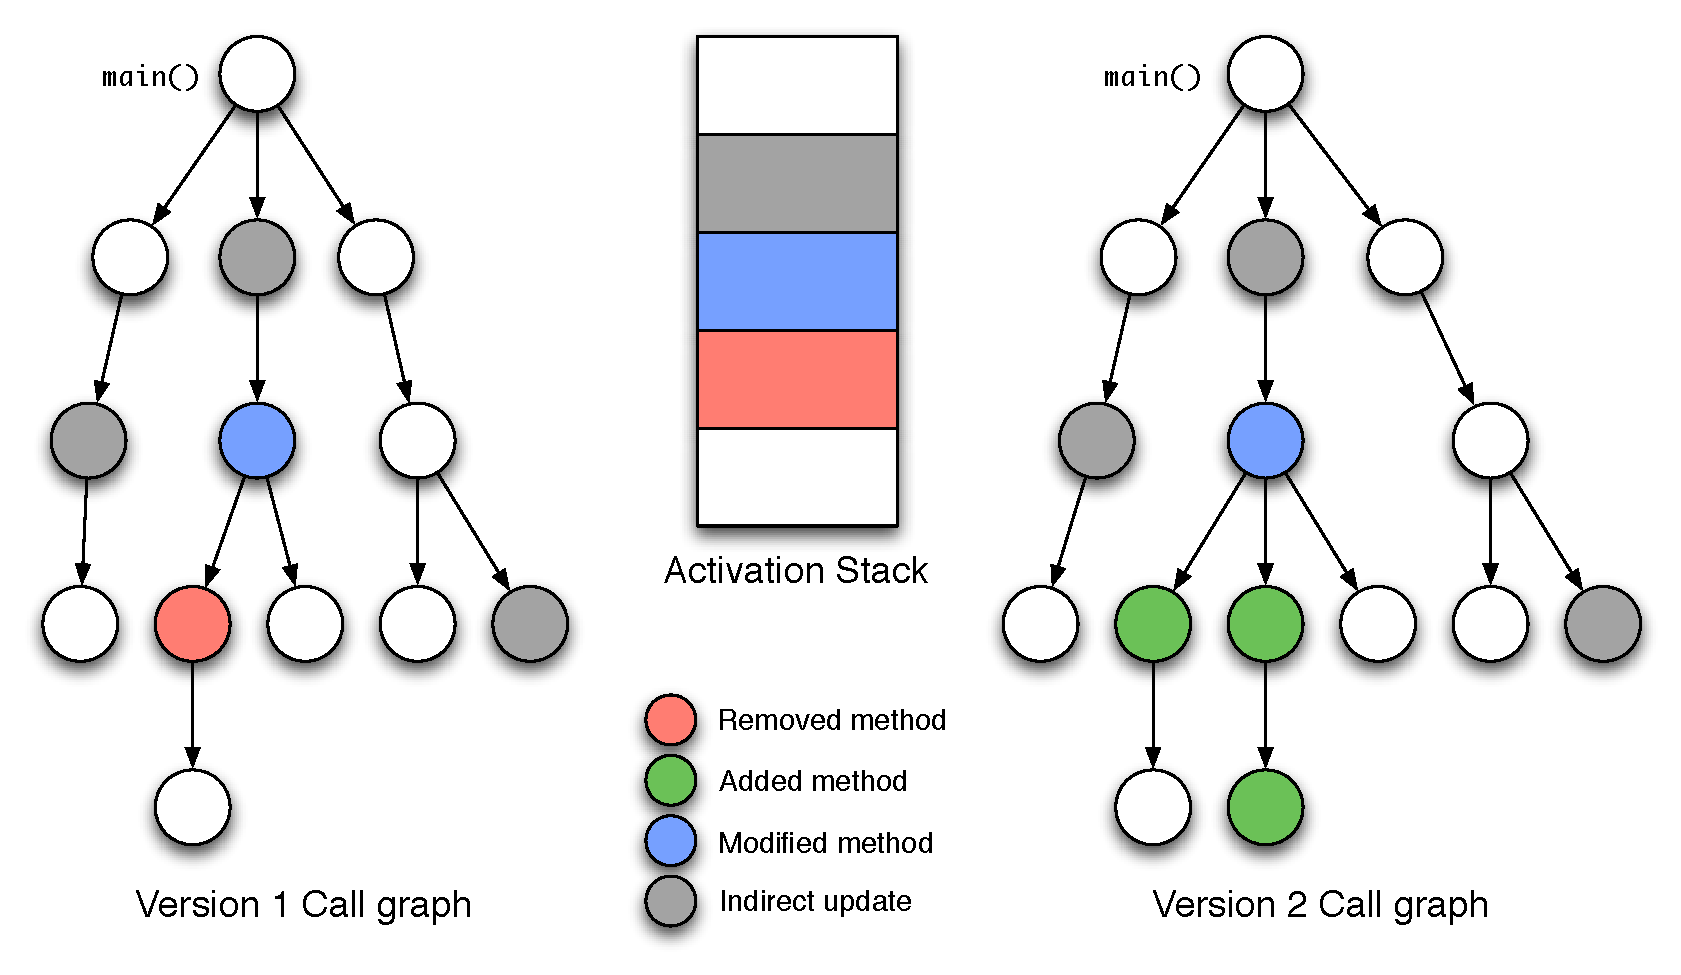
\includegraphics{images/safe-point-call-graph/both-call-graphs-2}}%
\uncover<3>{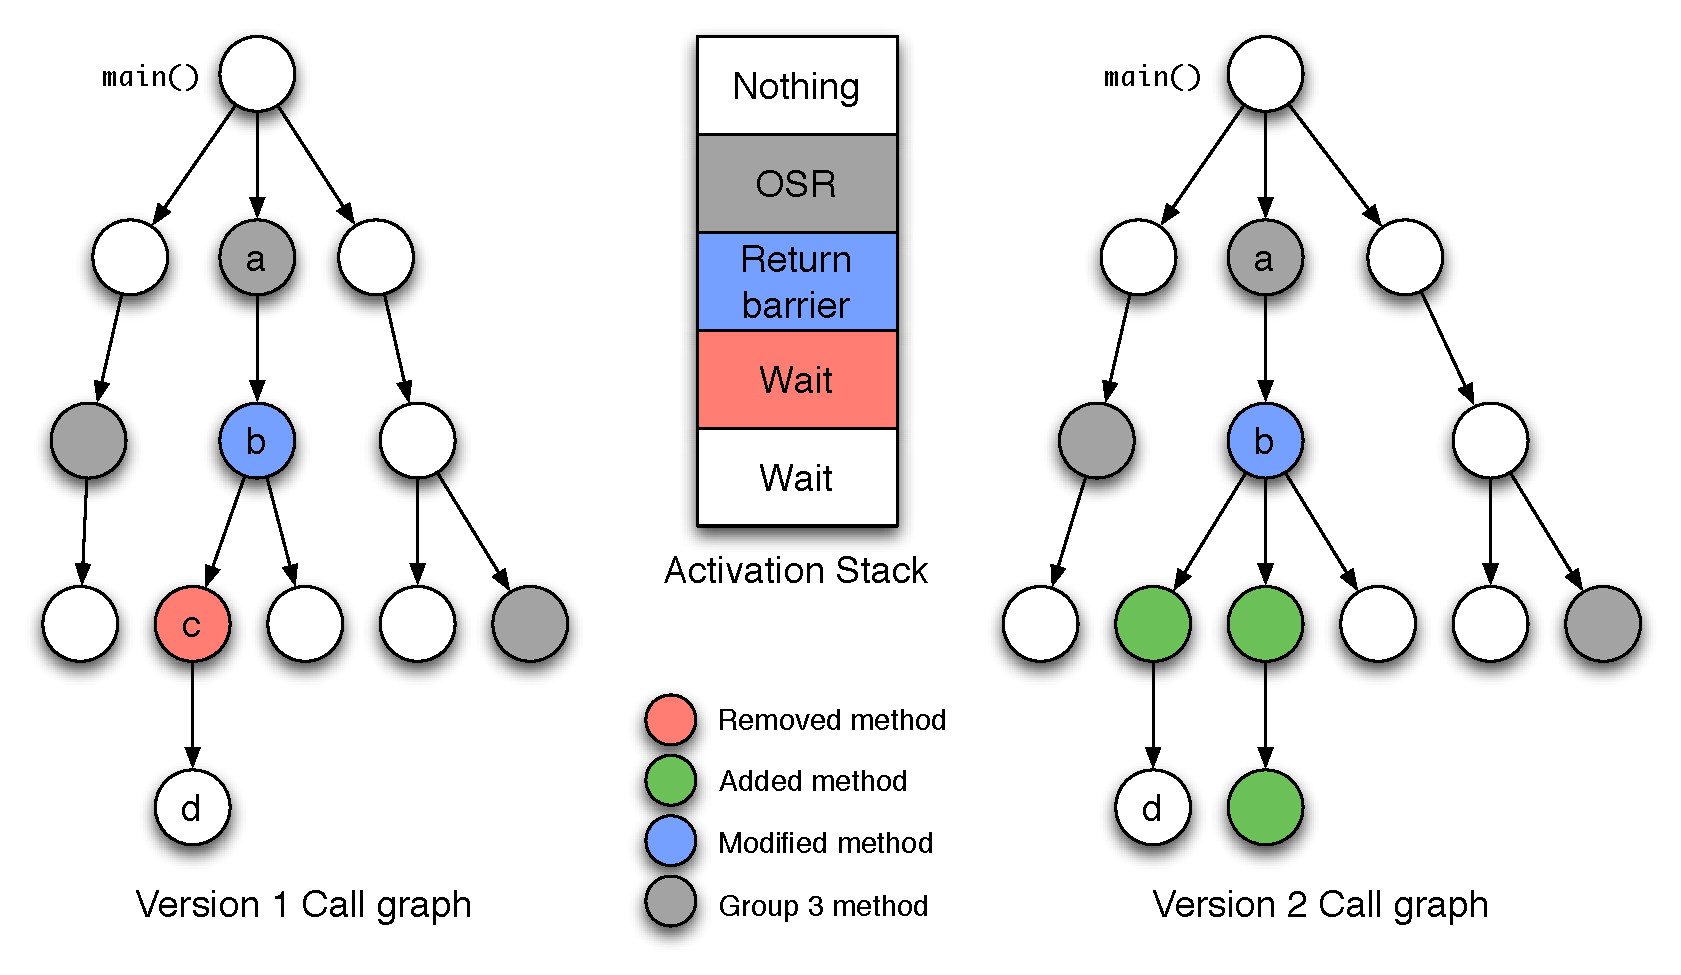
\includegraphics{images/safe-point-call-graph/both-call-graphs-3}}%
}
\end{frame}

% \begin{frame}[c,fragile]{Handling restricted methods}%{A Sub-title is optional}
% \hspace*{-5mm}
% \centering{\scalebox{0.67}{\includegraphics{images/flowchart}}}
% \end{frame}
% 
% \begin{frame}[t,fragile]{On stack replacement in \DSU{}}%{A Sub-title is optional}
% \begin{itemize}
% \item Used in \JikesRVM{} to optimize long running methods
% \item \DSU{} utilizes OSR for DSU
% \item Currently only support baseline-compiled methods
% \item Can OSR any method on stack
% \uncover<2>{
% \item Extract the state of the stack
% \item Construct a new method with a specialized prologue (at the bytecode
% level) that reconstructs the stack
% \item Last instruction of prologue jumps to bytecode where execution should
% resume from
% \item Overwrite the return address to point to the special method
% }
% \end{itemize}
% \end{frame}
% 
% 
% {
% \setbeamercovered{invisible}
% \begin{frame}[t,fragile]{OSR Example}%{A Sub-title is optional}
% \begin{footnotesize}
% \begin{columns}[t]
% 
% \begin{column}{0.4\paperwidth}
% \begin{semiverbatim}
% public class A \{
%   public int foo(int i, B b) \{
%     i = i + 1;
%     i = b.bar(i);
%     i = i + 1;
%     return i;
%   \}
% \}
% \end{semiverbatim}
% 
% \uncover<2-> {
% State: \\
% Thread: \#5 \\
% FP: 0x4ad33e40 \\
% PC: 9 \\
% Locals: i = 5, b = 0x52ae34a0 \\
% Stack vars: S0, S1, ... \\
% }
% \end{column}
% 
% \begin{column}{0.4\paperwidth}
% \begin{semiverbatim}
%  0 iload\_1
%  1 iconst\_1
%  2 iadd
%  3 istore\_1
%  4 aload\_2
%  5 iload\_1
%  6 invokevirtual <B.bar>
%  9 istore\_1
% 10 iload\_1
% 11 iconst\_1
% 12 iadd
% 13 istore\_1
% 14 iload\_1
% 15 ireturn
% \end{semiverbatim}
% \end{column}
% \end{columns}
% \end{footnotesize}
% \end{frame}
% }
% 
% {
% \setbeamercovered{invisible}
% \begin{frame}[t,fragile,shrink=20]{OSR Example}%{A Sub-title is optional}
% \begin{footnotesize}
% \begin{columns}[b]
% 
% \begin{column}{0.4\paperwidth}
% \begin{semiverbatim}
%  0 iload\_1
%  1 iconst\_1
%  2 iadd
%  3 istore\_1
%  4 aload\_2
%  5 iload\_1
%  6 invokevirtual <B.bar>
%  9 istore\_1
% 10 iload\_1
% 11 iconst\_1
% 12 iadd
% 13 istore\_1
% 14 iload\_1
% 15 ireturn
% \end{semiverbatim}
% \end{column}
% 
% \begin{column}{0.4\paperwidth}
% \begin{semiverbatim}
%    ldc 5
%    istore\_0 
%    ldc 0x52ae34a0
%    astore\_1
%    goto 9
%  0 iload\_1
%  1 iconst\_1
%  2 iadd
%  3 istore\_1
%  4 aload\_2
%  5 iload\_1
%  6 invokevirtual <B.bar>
%  9 istore\_1
% 10 iload\_1
% 11 iconst\_1
% 12 iadd
% 13 istore\_1
% 14 iload\_1
% 15 ireturn
% \end{semiverbatim}
% \end{column}
% 
% \end{columns}
% \end{footnotesize}
% \end{frame}
% }


\begin{frame}{Updating code}%{A Sub-title is optional}
\vspace*{-1mm}%
\hspace*{1mm}%
\includegraphics[scale=0.73]{images/process-state/both-process-state-arrow-highlight-code}%
\end{frame}

\begin{frame}[t,fragile,label=classload]{Installing new classes}%{A Sub-title is optional}
\JvolveTimeLine{}{}{current}{}{}
The VM maintains Class, Method and Field data structures
% \begin{itemize}
% \item The VM maintains Class, Method and Field data structures
% \item For Method updates: Only load the new method's bytecodes
% \item For Class updates: Rename the old class and load the entire class
% file (equivalent to have loaded two different class)
% \end{itemize}
\begin{center}
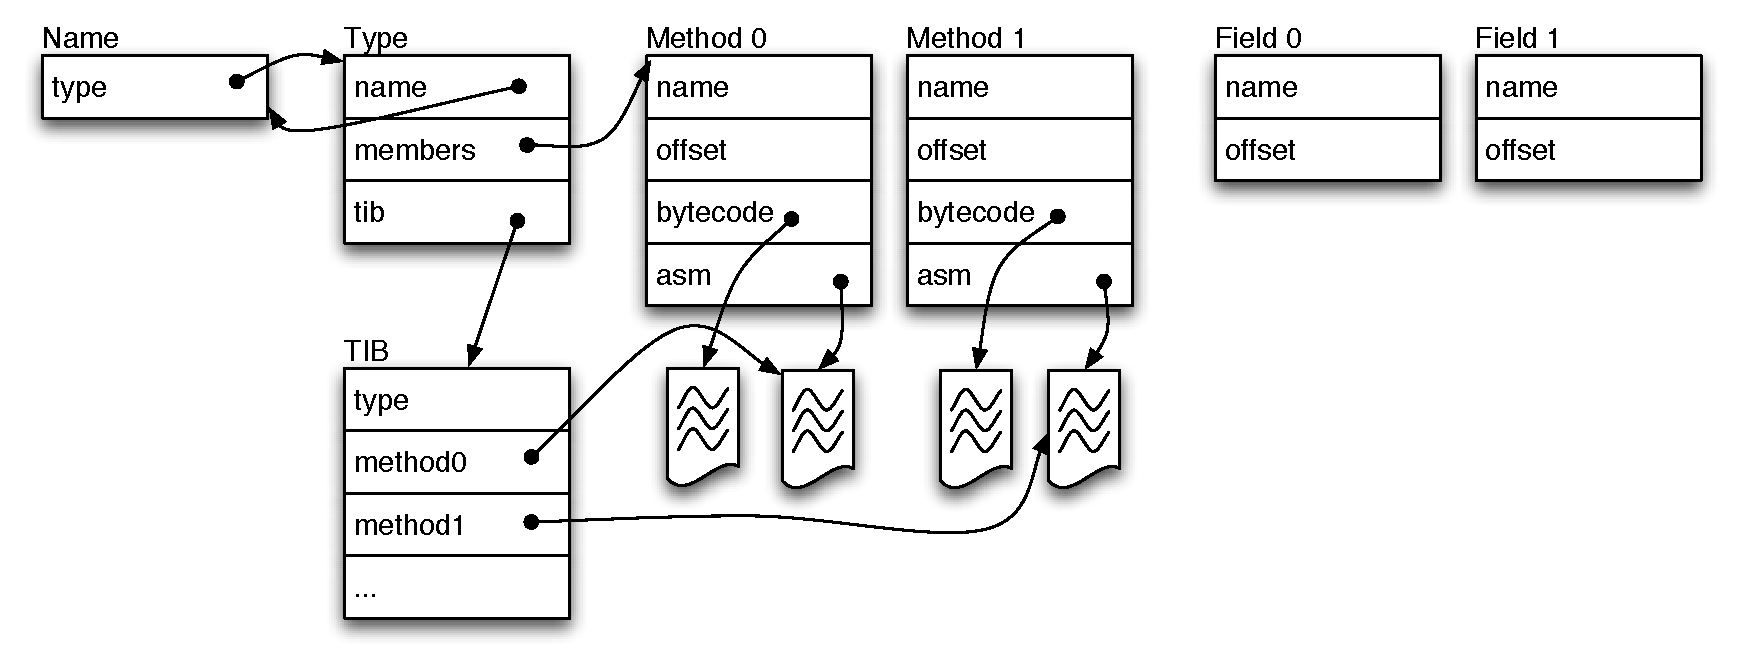
\includegraphics[scale=0.40]{images/vm-meta-data/vm-meta-data}%
\end{center}
\end{frame}

% \ifdraft{}{
% {
\setbeamertemplate{headline}{}
\setbeamertemplate{footline}{}
\setbeamertemplate{navigation symbols}{}
\setbeamercovered{invisible}
\begin{frame}[t,fragile]
\vspace*{-4ex}
\begin{tikzpicture}[auto]

\tikzstyle{title}=[font=\tiny\tt,text width=9mm,minimum height=4.5mm]
\tikzstyle{box}=[font=\tiny\tt,draw, thin,text width=9mm,minimum height=4.5mm,anchor=north west]
% Two rows
\newcommand{\HeaderRow}[2]{% name, content
\node [title] (#1 0) { #2 }; \\
}

\newcommand{\rowsTwo}[3]{% name, row0, row1
\HeaderRow{#1}{#2}
\node [box]   (#1 1) { #3 }; \\
}
% Three rows
\newcommand{\rowsThree}[4]{% name, row0, row1, row2
\rowsTwo{#1}{#2}{#3}
\node [box]   (#1 2) { #4 }; \\
}
% Four rows
\newcommand{\rowsFour}[5]{% name, row0, row1, row2
\rowsThree{#1}{#2}{#3}{#4}
\node [box]   (#1 3) { #5 }; \\
}
% Five rows
\newcommand{\rowsFive}[6]{% name, row0, row1, row2
\rowsFour{#1}{#2}{#3}{#4}{#5}
\node [box]   (#1 4) { #6 }; \\
}

\newcommand{\newRowsTwo}[3]{% name, row0, row1
\HeaderRow{#1}{#2}
\node [box,fill=new color]   (#1 1) { #3 }; \\
}
% Three rows
\newcommand{\newRowsThree}[4]{% name, row0, row1, row2
\newRowsTwo{#1}{#2}{#3}
\node [box,fill=new color]   (#1 2) { #4 }; \\
}
% Four rows
\newcommand{\newRowsFour}[5]{% name, row0, row1, row2
\newRowsThree{#1}{#2}{#3}{#4}
\node [box,fill=new color]   (#1 3) { #5 }; \\
}
% Five rows
\newcommand{\newRowsFive}[6]{% name, row0, row1, row2
\newRowsFour{#1}{#2}{#3}{#4}{#5}
\node [box,fill=new color]   (#1 4) { #6 }; \\
}

\newcommand{\metadataTwo}[4]{% name, position, contents 
\matrix [row sep=-0.4pt,anchor=north west] (#1) at #2 {
\rowsTwo{#1}{#3}{#4}
};}
\newcommand{\metadataThree}[5]{% name, position, contents 
\matrix [row sep=-0.4pt,anchor=north west] (#1) at #2 {
\rowsThree{#1}{#3}{#4}{#5}
};}
\newcommand{\metadataFour}[6]{% name, position, contents 
\matrix [row sep=-0.4pt,anchor=north west] (#1) at #2 {
\rowsFour{#1}{#3}{#4}{#5}{#6}
};}
\newcommand{\metadataFive}[7]{% name, position, contents 
\matrix [row sep=-0.4pt,anchor=north west] (#1) at #2 {
\rowsFive{#1}{#3}{#4}{#5}{#6}{#7}
};}

\newcommand{\newMetadataTwo}[4]{% name, position, contents 
\matrix [row sep=-0.4pt,anchor=north west] (#1) at #2 {
\newRowsTwo{#1}{#3}{#4}
};}
\newcommand{\newMetadataThree}[5]{% name, position, contents 
\matrix [row sep=-0.4pt,anchor=north west] (#1) at #2 {
\newRowsThree{#1}{#3}{#4}{#5}
};}
\newcommand{\newMetadataFour}[6]{% name, position, contents 
\matrix [row sep=-0.4pt,anchor=north west] (#1) at #2 {
\newRowsFour{#1}{#3}{#4}{#5}{#6}
};}
\newcommand{\newMetadataFive}[7]{% name, position, contents 
\matrix [row sep=-0.4pt,anchor=north west] (#1) at #2 {
\newRowsFive{#1}{#3}{#4}{#5}{#6}{#7}
};}

\colorlet{new color}{green!40}
\tikzstyle{line}=[draw, thin, -latex',]
\tikzstyle{every path}=[line]

\begin{scope}
  \metadataTwo{typeref}{(0,-1)}{Name}{type}
  \uncover<4->{ \newMetadataTwo{typerefnew}{(0,0)}{Name}{type} }
  \metadataFour{class}{(2,0)}{Type}{name}{members}{tib}
  \metadataThree{field}{(4,0)}{Field}{name}{offset}
  \node at (5.75,-0.75) {...};
  \metadataFive{method}{(6,0)}{Method}{name}{offset}{bytecode}{asm}
  \metadataFive{tib}{(4,-1.5)}{TIB}{type}{method0}{method1}{...}
  \uncover<-2>{ \node[box,text width=14mm] (bc) at (8,-1)   { 0100100101...  }; }
  \node[box,text width=14mm] (mc) at (8,-2)   { 1010000111... };
  \uncover<2> { \node[box,text width=14mm,fill=new color] (bcnew) at (8,-0.25) { 1100100101... }; }
  \uncover<3->{ \node[box,text width=14mm] (bcnew) at (8,-0.25) { 1100100101... }; }
\end{scope}

\uncover<-3> { \path (typeref 1.east) to [out=0,in=180] (class 1.north west); }
\uncover<-3> { \path (class 1.west)   to [out=180,in=0] (typeref 1.south east); }
\uncover<4-> { \path (typerefnew 1.east) to [out=0,in=180] (class 1.north west); }
\uncover<4-> { \path (class 1.west)   to [out=180,in=0] (typerefnew 1.south east); }
\path (class 2.east)         to [out=0,in=180]   (field 1.north west);
\path (class 3.east)         to [out=0,in=135]   (tib 1.north west);
\path (tib 1.west)           to [out=180,in=315] (class 3.south);
\path (tib 2.east)           to [out=0,in=225]   (mc.south west);
\path (method 4.east)        to                  (mc.north west);
\uncover<1>  { \path (method 3.east)        to   (bc.north west);    }
\uncover<2-> { \path (method 3.east)        to   (bcnew.north west); }

\uncover<5->{
\begin{scope}[yshift=-4.5cm]
  \newMetadataFour{class1}{(2,0)}{Type}{name}{members}{tib}
  \newMetadataThree{field1}{(4,0)}{Field}{name}{offset}
  \node at (5.75,-0.75) {...};
  \newMetadataFive{method1}{(6,0)}{Method}{name}{offset}{bytecode}{asm}
  \newMetadataFive{tib1}{(4,-1.5)}{TIB}{type}{method0}{method1}{...}
  \node[box,text width=14mm,fill=new color] (bc1) at (8,-1) { 0100100101... };
  \node[box,text width=14mm,fill=new color] (mc1) at (8,-2) { 1010000111... };
\end{scope}
  \path (class1 2.east)         to [out=0,in=180]   (field1 1.north west);
  \path (class1 3.east)         to [out=0,in=135]   (tib1 1.north west);
  \path (tib1 2.east)           to [out=0,in=225]   (mc1.south west);
  \path (tib1 1.west)           to [out=180,in=315] (class1 3.south);
  \path (method1 3.east)        to                  (bc1.north west);
  \path (method1 4.east)        to                  (mc1.north west);
  \path (class1 1.north west)   to                  (typeref 1.south east);
  \path (typeref 1.south)       to [out=285,in=180] (class1 1.west);
}

\end{tikzpicture}
\end{frame}
}

% }

\begin{frame}{Updating a method}%{A Sub-title is optional}
\vspace*{-1mm}%
\begin{center}
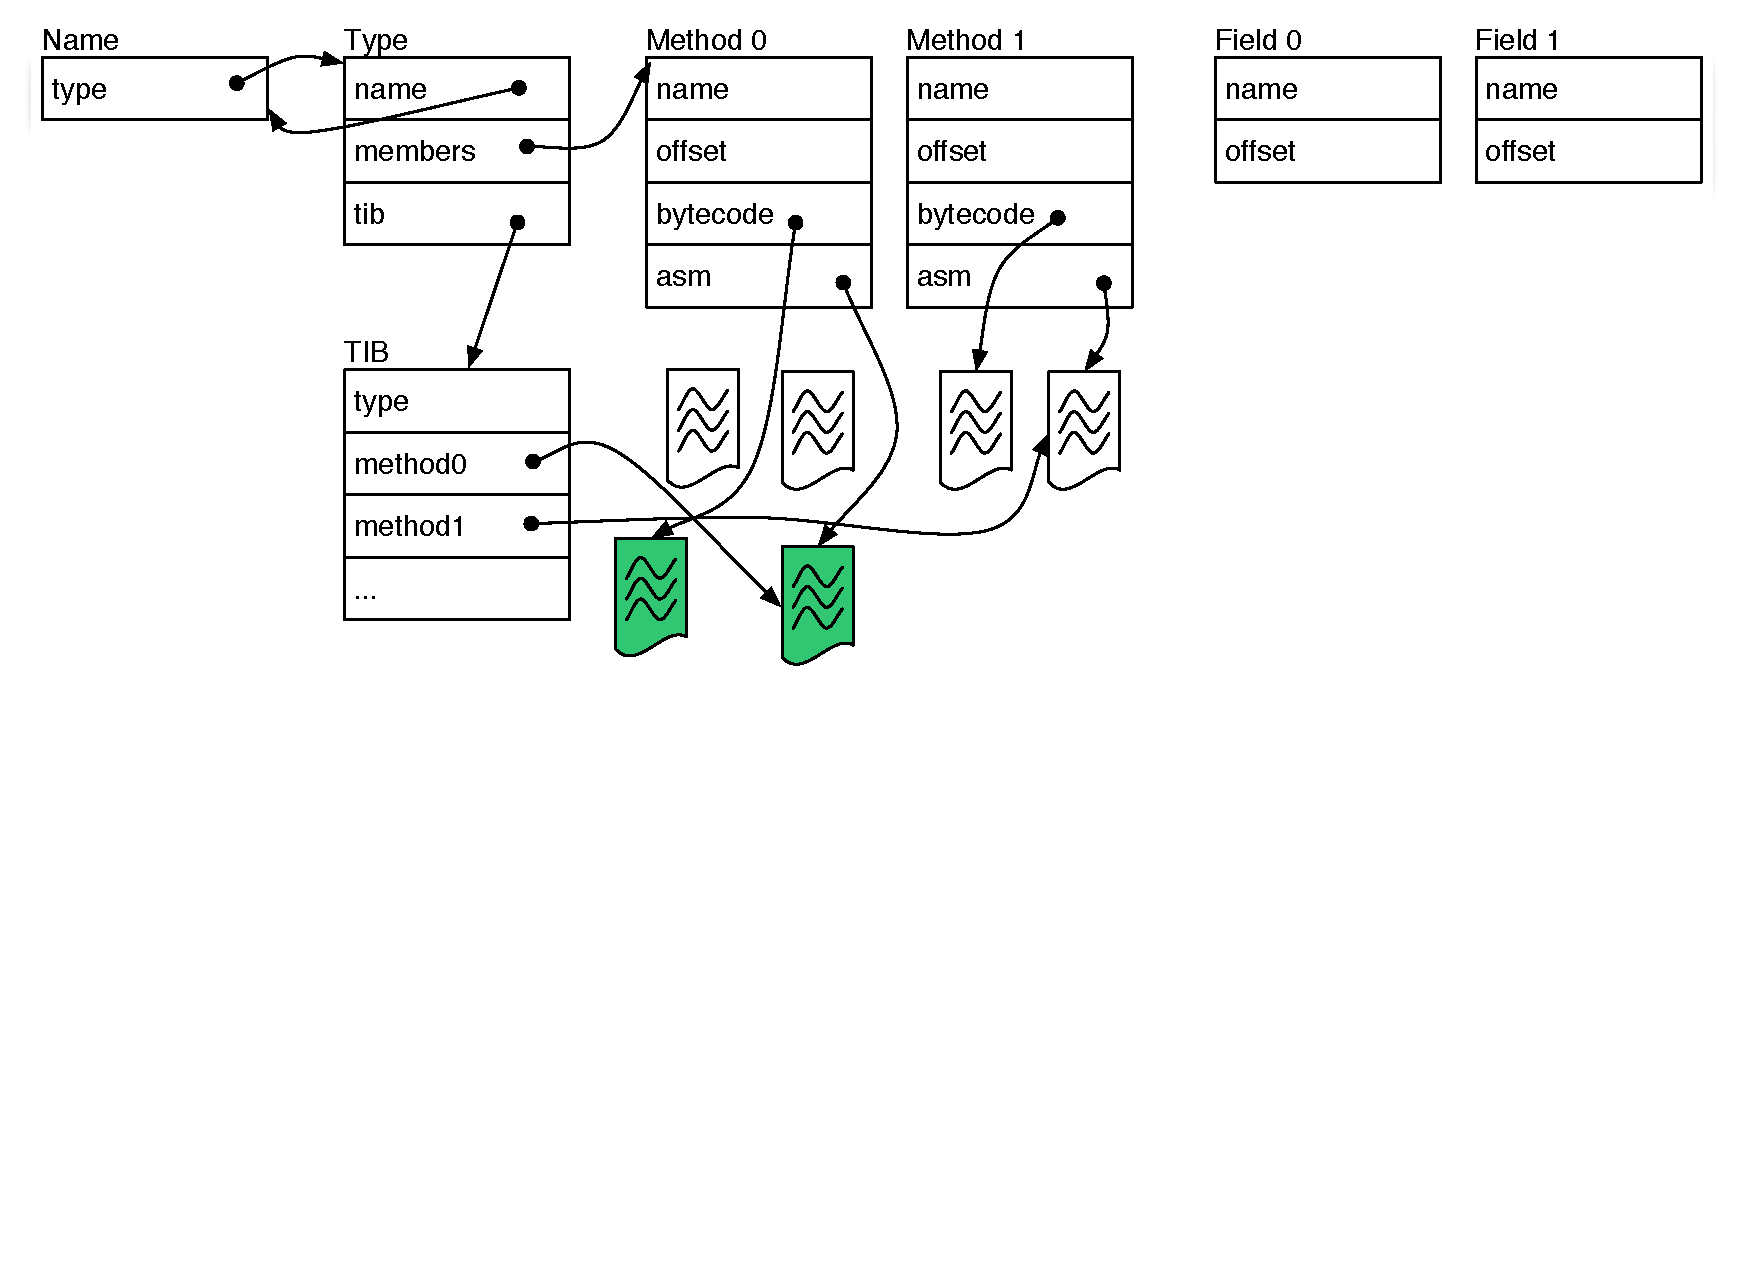
\includegraphics[scale=0.36]{images/vm-meta-data/vm-meta-data-updated-method}%
\end{center}
\end{frame}

\begin{frame}{Updating a class}%{A Sub-title is optional}
\vspace*{-1mm}%
\begin{center}
\includegraphics[scale=0.36]<1>{images/vm-meta-data/vm-meta-data-renamed-class}%
\includegraphics[scale=0.36]<2>{images/vm-meta-data/vm-meta-data-updated-class}%
\end{center}
\end{frame}

\begin{frame}{Updating heap data}%{A Sub-title is optional}
\vspace*{-1mm}%
\hspace*{1mm}%
\includegraphics[scale=0.73]{images/process-state/both-process-state-arrow-highlight-heap}%
\end{frame}

\begin{frame}[t,fragile,label=transform]{Transforming objects}%{A Sub-title is optional}
\JvolveTimeLine{}{}{}{current}{}
\begin{itemize}
\item Supported on top of a semi-space copying collector
\item As part of collector's visit allocate additional space for updated
      objects
\item After GC, run class and object transformers
\end{itemize}
\end{frame}

\ifdraft{}{

%%%%%%%%%%%%%%%%%%%%%%%%%%%%%%%%%%%%%%%%%%%%%%%%%%%%%%%%%%%%%%%%%%%%%%%%
% Colors
\colorlet{black object color}{black!60}
\colorlet{grey object color}{black!20}
\colorlet{forwarding pointer color}{structure.fg!40}
\colorlet{dsu v0 color}{blue!60}
\colorlet{dsu v1 empty color}{blue!20}
\colorlet{dsu forwarding pointer color}{forwarding pointer color!50!dsu v0 color}
%%%%%%%%%%%%%%%%%%%%%%%%%%%%%%%%%%%%%%%%%%%%%%%%%%%%%%%%%%%%%%%%%%%%%%%%

%%%%%%%%%%%%%%%%%%%%%%%%%%%%%%%%%%%%%%%%%%%%%%%%%%%%%%%%%%%%%%%%%%%%%%%%
% Define the style for each field of the object
\newlength{\drawthickness}
\setlength{\drawthickness}{0.6pt}
\newlength{\fielddimension}
\setlength{\fielddimension}{5mm}
\tikzstyle{field}=[
    rectangle,
    draw=black,
    line width=\drawthickness,
    minimum width=\fielddimension,
    minimum height=\fielddimension,
    inner sep=0pt,
    font=\tiny,
]
\tikzstyle{new space grey field}=[field,fill=grey object color]
\tikzstyle{new space black field}=[field,fill=black object color]
\tikzstyle{dsu v0 field}=[field,fill=dsu v0 color]
\tikzstyle{dsu v1 empty field}=[field,fill=dsu v1 empty color]
%%%%%%%%%%%%%%%%%%%%%%%%%%%%%%%%%%%%%%%%%%%%%%%%%%%%%%%%%%%%%%%%%%%%%%%%

%%%%%%%%%%%%%%%%%%%%%%%%%%%%%%%%%%%%%%%%%%%%%%%%%%%%%%%%%%%%%%%%%%%%%%%%
% Define the style for each object
\tikzstyle{object}=[
    column sep=-\drawthickness,
    nodes=field,
    inner sep=0pt,
]
\tikzstyle{new space grey object}=[object,nodes=new space grey field]
\tikzstyle{new space black object}=[object,nodes=new space black field]
\tikzstyle{dsu v0 object}=[object,nodes=dsu v0 field]
\tikzstyle{dsu v1 empty object}=[object,nodes=dsu v1 empty field]
%%%%%%%%%%%%%%%%%%%%%%%%%%%%%%%%%%%%%%%%%%%%%%%%%%%%%%%%%%%%%%%%%%%%%%%%

%%%%%%%%%%%%%%%%%%%%%%%%%%%%%%%%%%%%%%%%%%%%%%%%%%%%%%%%%%%%%%%%%%%%%%%%
% Style for arrows
\tikzstyle{regular}=[-to,draw]
\tikzstyle{transparent}=[-to,draw=black!15!bg]
%%%%%%%%%%%%%%%%%%%%%%%%%%%%%%%%%%%%%%%%%%%%%%%%%%%%%%%%%%%%%%%%%%%%%%%%

%%%%%%%%%%%%%%%%%%%%%%%%%%%%%%%%%%%%%%%%%%%%%%%%%%%%%%%%%%%%%%%%%%%%%%%%
% Define a macro for creating an object with two fields
\newcommand{\twoFieldsObject}[3]{% name, position, object style
\matrix[#3,ampersand replacement=\&] (#1) at #2 {
  \node (#1 0) {}; \& \node (#1 1) {}; \\
};}
\newcommand{\fourFieldsObject}[3]{% name, position, object style
\matrix[#3,ampersand replacement=\&] (#1) at #2 {
  \node (#1 0) {}; \& \node (#1 1) {}; \& \node (#1 2) {}; \& \node (#1 3) {}; \\
};}


% Command to write a label next to an object
\newcommand{\labelObject}[4]{% label text, object name, label position, label anchor
\draw (#2.#3) node[anchor=#4,inner sep=0.5pt,font=\tiny] {#1};}
\newcommand{\oldSpaceLabelObject}[2]{% label text, object name
\labelObject{#1}{#2}{north west}{north east}}
\newcommand{\newSpaceLabelObject}[2]{% label text, object name
\labelObject{#1}{#2}{150}{south west}}

\newcommand{\oldSpaceObject}[3][object]{% object style, name, position
\twoFieldsObject{#2}{#3}{#1}\oldSpaceLabelObject{#2}{#2}}
\newcommand{\dsuOldSpaceVersionZeroObject}[2]{% name, location
\twoFieldsObject{#1}{#2}{dsu v0 object}\oldSpaceLabelObject{#1 $v_0$}{#1}}
\newcommand{\dsuOldSpaceVersionOneObject}[2]{% name, location
\fourFieldsObject{#1 v1}{#2}{dsu v1 empty object}\oldSpaceLabelObject{#1 $v_1$}{#1 v1}}

\newcommand{\newSpaceObject}[4][]{% extra name, name, position, object style
\twoFieldsObject{#2}{#3}{#4}\newSpaceLabelObject{#2#1}{#2}}
\newcommand{\newSpaceVersionOneEmptyObject}[2]{% name, position
\fourFieldsObject{#1 v1}{#2}{dsu v1 empty object}\labelObject{#1 $v_1$}{#1 v1}{165}{south west}}
\newcommand{\newSpaceGreyObject}[2]{% name, position
\newSpaceObject{#1}{#2}{new space grey object}}
\newcommand{\newSpaceBlackObject}[2]{% name, position
\newSpaceObject{#1}{#2}{new space black object}}
\newcommand{\dsuNewSpaceGreyObject}[2]{% name, position
\newSpaceObject[\ $v_0$]{#1}{#2}{new space grey object}}
\newcommand{\dsuNewSpaceBlackObject}[2]{% name, position
\newSpaceObject[\ $v_0$]{#1}{#2}{new space black object}}

\newcommand{\forwardingPointer}[1]{% name
\node[field,minimum width=2\fielddimension,fill=forwarding pointer color] at (#1.center) {#1'};
}
\newcommand{\dsuForwardingPointer}[1]{% name
\node[field,minimum width=2\fielddimension,fill=dsu forwarding pointer color] at (#1.center) {#1' $v_1$};
}
%%%%%%%%%%%%%%%%%%%%%%%%%%%%%%%%%%%%%%%%%%%%%%%%%%%%%%%%%%%%%%%%%%%%%%%%

%%%%%%%%%%%%%%%%%%%%%%%%%%%%%%%%%%%%%%%%%%%%%%%%%%%%%%%%%%%%%%%%%%%%%%%%
% Define coordinates of the various objects
\newcommand{\objectRoot}{(-3,0.8)}
\newcommand{\objectA}{(0,0)}
\newcommand{\objectB}{(-2,-1)}
\newcommand{\objectC}{(2,-1)}
\newcommand{\objectD}{(-3,-2)}
\newcommand{\objectE}{(-1,-2)}
\newcommand{\objectF}{(1,-2)}
\newcommand{\objectG}{(3,-2)}

\newcommand{\objectAprime}{(-3.5,0.25)}
\newcommand{\objectBprime}{(-2.5,0.25)}
\newcommand{\objectCprime}{(-1.5,0.25)}
\newcommand{\objectDprime}{(-0.5,0.25)}
\newcommand{\objectEprime}{(+0.5,0.25)}
\newcommand{\objectFprime}{(+1.5,0.25)}
\newcommand{\objectGprime}{(+2.5,0.25)}

% old space
\newcommand{\objectCVersionOne}{(2.5,0)}
\newcommand{\objectFVersionOne}{(1,-3)}
% new space
\newcommand{\objectCprimeVersionOne}{(-3,-1.75)}
\newcommand{\objectFprimeVersionOne}{(-0.75,-1.75)}
%%%%%%%%%%%%%%%%%%%%%%%%%%%%%%%%%%%%%%%%%%%%%%%%%%%%%%%%%%%%%%%%%%%%%%%%

% vim:tw=0:nospell

% 
% The various steps of the animation are
% Slide 1: Show all objects
% Slide 2: A is copied
% Slide 3: A is scanned; B, C are copied
% Slide 4: A, B are scanned; C, D, E are copied
% Slide 5: A, B, C are scanned; D, E, F, G are copied
% Slide 6: A-D are scanned
% Slide 7: A-E are scanned
% Slide 8: A-F are scanned
% Slide 9: A-G are scanned
{
\begin{frame}[fragile]{Semi-space copying collector}%{A Sub-title is optional}
\setbeamercovered{invisible}
\begin{columns}[t]
\begin{column}[T]{0.67\paperwidth}
\begin{tikzpicture}
\begin{scope}
  % objects
  \uncover<1>{       \node[field] (root) at \objectRoot {root};                        }
  \uncover<2->{      \node[new space black field] (root) at \objectRoot {root};        }
                     \oldSpaceObject{A}{\objectA}
                     \oldSpaceObject{B}{\objectB}
                     \oldSpaceObject{C}{\objectC}
                     \oldSpaceObject{D}{\objectD}
                     \oldSpaceObject{E}{\objectE}
                     \oldSpaceObject{F}{\objectF}
                     \oldSpaceObject{G}{\objectG}
  % forwarding pointers
  \uncover<2->{      \forwardingPointer{A}                             }
  \uncover<3->{      \forwardingPointer{B}
                     \forwardingPointer{C}                             }
  \uncover<4->{      \forwardingPointer{D}
                     \forwardingPointer{E}                             }
  \uncover<5->{      \forwardingPointer{F}
                     \forwardingPointer{G}                             }
  % pointer arrows
  \uncover<1>   {    \path[regular]     (root.east)  to [out=330,in=120] (A.140)    ;          }
  \uncover<1>   {    \path[regular]     (A 0.center) to                (B.90)     ;            }
  \uncover<1>   {    \path[regular]     (A 1.center) to                (C.135)    ;            }
  \uncover<1-2> {    \path[regular]     (B 0.center) to                (D.135)    ;            }
  \uncover<1-2> {    \path[regular]     (B 1.center) to                (E.90)     ;            }
  \uncover<1-2> {    \path[regular]     (C 0.center) to                (F.135)    ;            }
  \uncover<1-2> {    \path[regular]     (C 1.center) to                (G.90)     ;            }
  \uncover<1-4> {    \path[regular]     (F 0.center) to                (A)        ;            }
                                                                      
  \uncover<2> {    \path[transparent]   (root.east)  to [out=0,in=120] (A.140)    ;            }
  \uncover<2> {    \path[transparent]   (A 0.center) to                (B.90)     ;            }
  \uncover<2> {    \path[transparent]   (A 1.center) to                (C.135)    ;            }
  \uncover<3> {    \path[transparent]   (B 0.center) to                (D.135)    ;            }
  \uncover<3> {    \path[transparent]   (B 1.center) to                (E.90)     ;            }
  \uncover<3> {    \path[transparent]   (C 0.center) to                (F.135)    ;            }
  \uncover<3> {    \path[transparent]   (C 1.center) to                (G.90)     ;            }
  \uncover<5> {    \path[transparent]   (F 0.center) to                (A)        ;            }

  \draw[draw,thin] (-4,-2.5) rectangle (4,0.5);
  \draw (4,0.5) node[anchor=north east,inner sep=1pt,font=\tiny] {FromSpace};

\end{scope}
\begin{scope}[yshift=-3.75cm]
  % objects
  \uncover<2>   {    \newSpaceGreyObject{A'}{\objectAprime}                          }
  \uncover<3->  {    \newSpaceBlackObject{A'}{\objectAprime}                         }

  \uncover<3>   {    \newSpaceGreyObject{B'}{\objectBprime}                          }
  \uncover<4->  {    \newSpaceBlackObject{B'}{\objectBprime}                         }

  \uncover<3-4> {    \newSpaceGreyObject{C'}{\objectCprime}                          }
  \uncover<5->  {    \newSpaceBlackObject{C'}{\objectCprime}                         }

  \uncover<4-5> {    \newSpaceGreyObject{D'}{\objectDprime}                          }
  \uncover<6->  {    \newSpaceBlackObject{D'}{\objectDprime}                         }

  \uncover<4-6> {    \newSpaceGreyObject{E'}{\objectEprime}                          }
  \uncover<7->  {    \newSpaceBlackObject{E'}{\objectEprime}                         }

  \uncover<5-7> {    \newSpaceGreyObject{F'}{\objectFprime}                          }
  \uncover<8->  {    \newSpaceBlackObject{F'}{\objectFprime}                         }

  \uncover<5-8> {    \newSpaceGreyObject{G'}{\objectGprime}                          }
  \uncover<9->  {    \newSpaceBlackObject{G'}{\objectGprime}                         }

  % pointer arrows
  \uncover<2->  {    \path[regular] (root.west)   to [out=220,in=95] (A'.north west);    }
  \uncover<2>   {    \path[regular] (A' 0.center) to [out=130,in=180] (B.west);
                     \path[regular] (A' 1.center) to [out=70,in=180]  (C.west);           }
  \uncover<3->  {    \path[regular] (A' 0.center) to [out=80,in=135]  (B'.150);          
                     \path[regular] (A' 1.center) to [out=70,in=150]  (C'.150);           }
                                                                                         
  \uncover<3>   {    \path[regular] (B' 0.center) to                  (D.south);         
                     \path[regular] (B' 1.center) to                  (E.south);          }
  \uncover<4->  {    \path[regular] (B' 0.center) to [out=300,in=240] (D'.215);          
                     \path[regular] (B' 1.center) to [out=330,in=240] (E'.215);           }
                                                                                         
  \uncover<3-4> {    \path[regular] (C' 0.center) to                  (F.south);         
                     \path[regular] (C' 1.center) to                  (G.south west);     }
  \uncover<5->  {    \path[regular] (C' 0.center) to [out=80,in=135]  (F'.150);          
                     \path[regular] (C' 1.center) to [out=70,in=150]  (G'.150);           }
                                                                                         
  \uncover<5-7> {    \path[regular] (F' 0.center) to [out=30,in=325]  (A);                }
  \uncover<8->  {    \path[regular] (F' 0.center) to [out=215,in=330] (A'.215);           }

  % transparent arrows
  \uncover<3>   {    \path[transparent] (A' 0.center) to [out=130,in=180] (B.west);
                     \path[transparent] (A' 1.center) to [out=70,in=180]  (C.west);       }

  \uncover<4>   {    \path[transparent] (B' 0.center) to                  (D.south);
                     \path[transparent] (B' 1.center) to                  (E.south);      }

  \uncover<5>   {    \path[transparent] (C' 0.center) to                  (F.south);
                     \path[transparent] (C' 1.center) to                  (G.south west); }

  \uncover<8>   {    \path[transparent] (F' 0.center) to [out=30,in=325]  (A);            }
  

  \draw[draw,thin] (-4,-2) rectangle (4,0.5);
  \draw (4,-2) node[anchor=south east,inner sep=1pt,font=\tiny] {ToSpace};
\end{scope}
\end{tikzpicture}
\end{column}
\begin{column}[T]{0.25\paperwidth}
\begin{block}{}
\begin{tikzpicture}
\tikzstyle{column 2}=[anchor=west]
\matrix [row sep=0.5ex] {
\node[new space grey field] {};                & \node {\tiny Visited}; \\
\node[new space black field] {};               & \node {\tiny All children visited}; \\
\node[field,fill=forwarding pointer color] {}; & \node {\tiny Forwarding pointer}; \\
};
\end{tikzpicture}
\end{block}

\begin{block}{}
\begin{scriptsize}
\only<1>{
The heap is divided into two spaces. Only one space is used by the
application. The garbage collector copies objects from \emph{FromSpace} to
\emph{ToSpace}.
}
\only<2>{
GC copies A to \emph{ToSpace}, leaves a forwarding pointer pointing to the
new copy A'.
}
\only<3>{
GC scans A'. The objects pointed to by A' (B and C) are copied to
\emph{ToSpace}. A's fields point to the copied objects.
}
\only<4>{
Next, the GC scans B', and copies objects D and E.
}
\only<5-7>{
Similarly for C'\uncover<6-7>{, D'}\uncover<7>{, and E.}
}
\only<8>{
When scanning F', the first field points to A in \emph{FromSpace}, which is a
forwarding pointer. After the scan, this field points to A'.
}
\only<9>{
All objects in \emph{ToSpace} are scanned. All reachable/live objects are now
in \emph{ToSpace}.
}
\end{scriptsize}
\end{block}
\end{column}
\end{columns}
\end{frame}
}

% vim:tw=0:nospell

}

\begin{frame}{Transforming objects}%{A Sub-title is optional}
\vspace*{-1mm}%
\begin{center}%
\only<1>{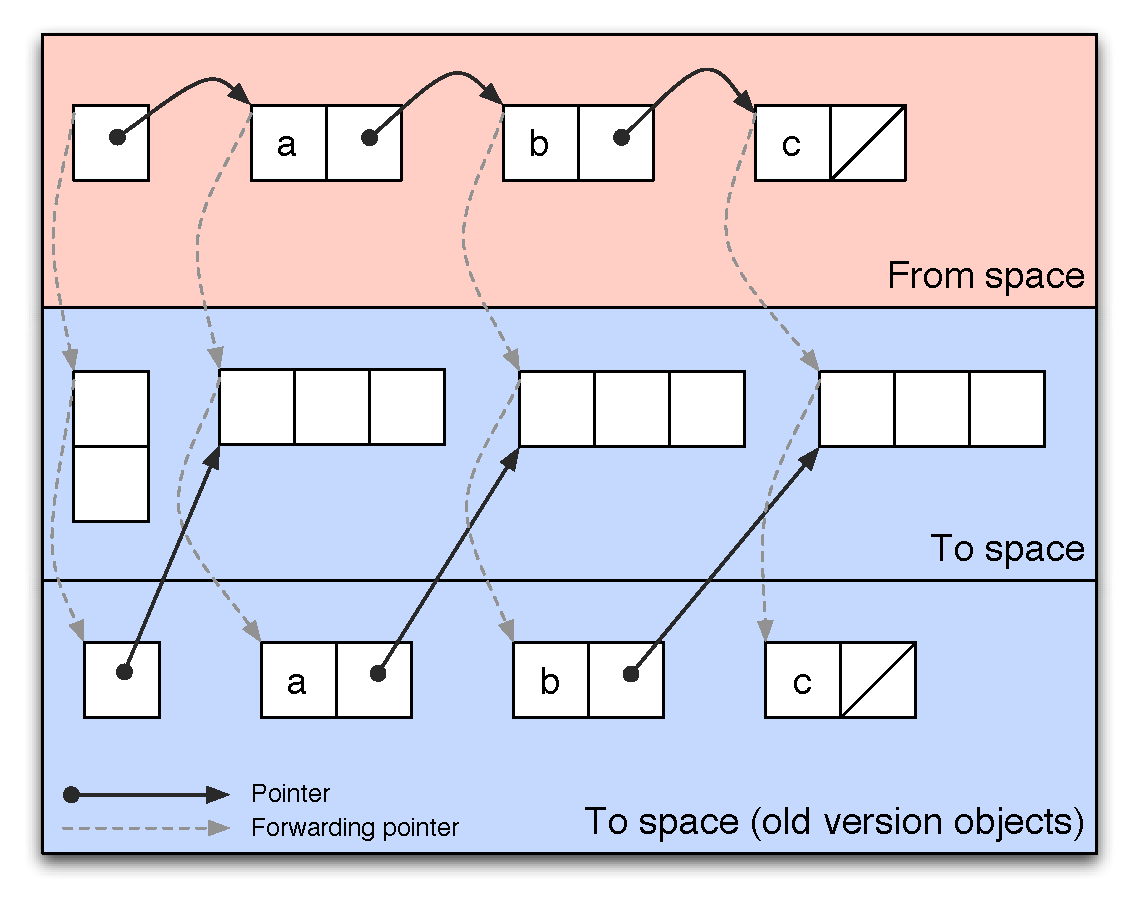
\includegraphics[scale=0.51]{images/singly-doubly/singly-doubly}}%
\only<2>{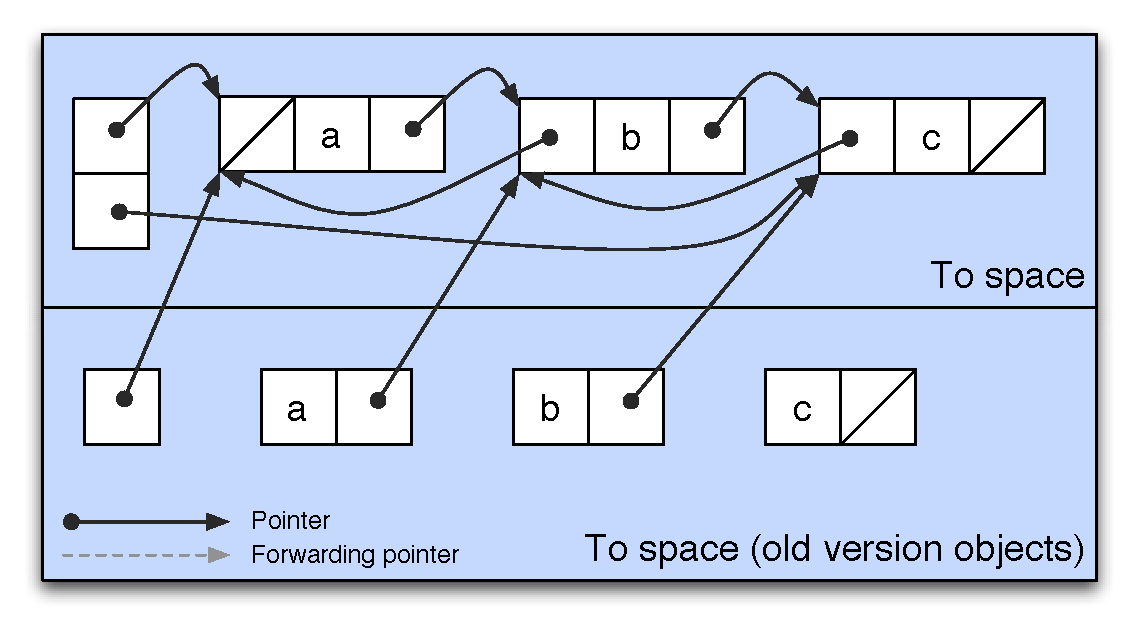
\includegraphics[scale=0.51]{images/singly-doubly/singly-doubly-transformed}}%
\only<3>{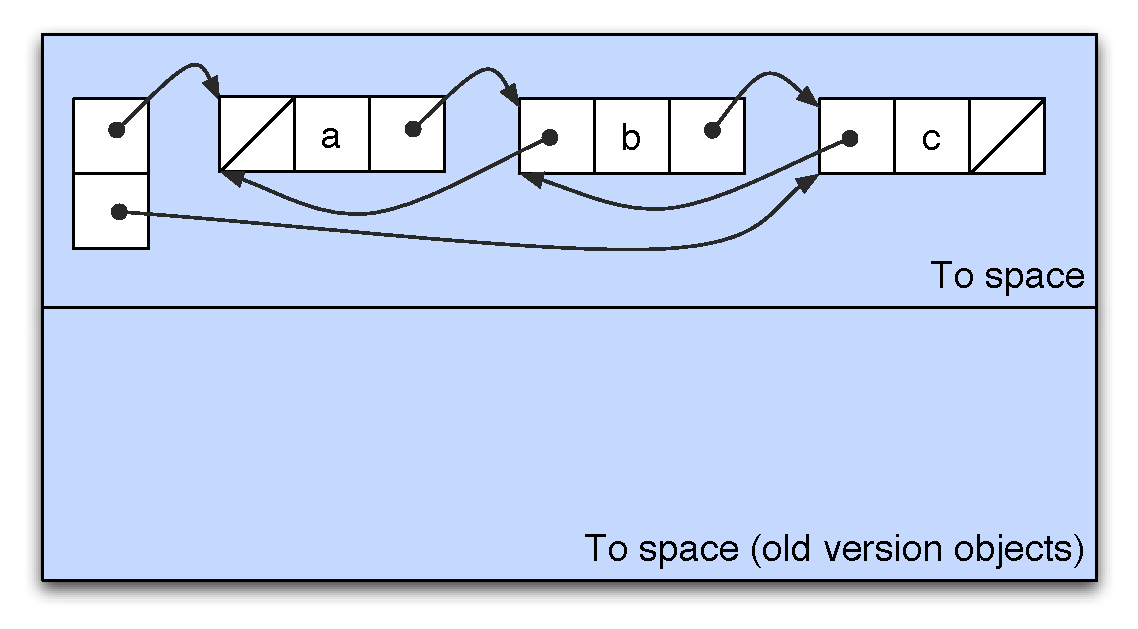
\includegraphics[scale=0.51]{images/singly-doubly/singly-doubly-transformed-final}}%
\end{center}%
\end{frame}

\begin{frame}[fragile]{Transforming objects}%{A Sub-title is optional}
\begin{columns}[c]
\begin{column}{0.7\paperwidth}
\only<1>{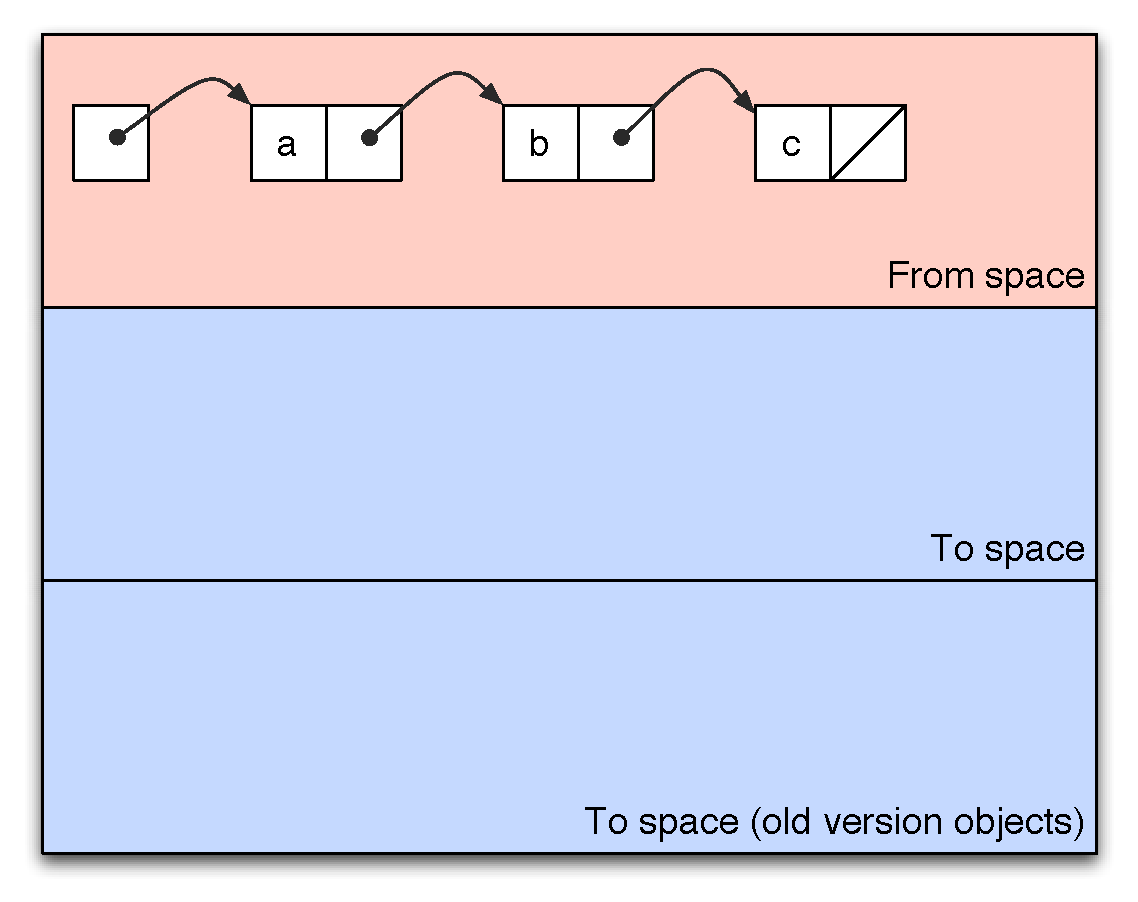
\includegraphics[scale=0.45]{images/singly-doubly/before-gc-copy}}%
\only<1>{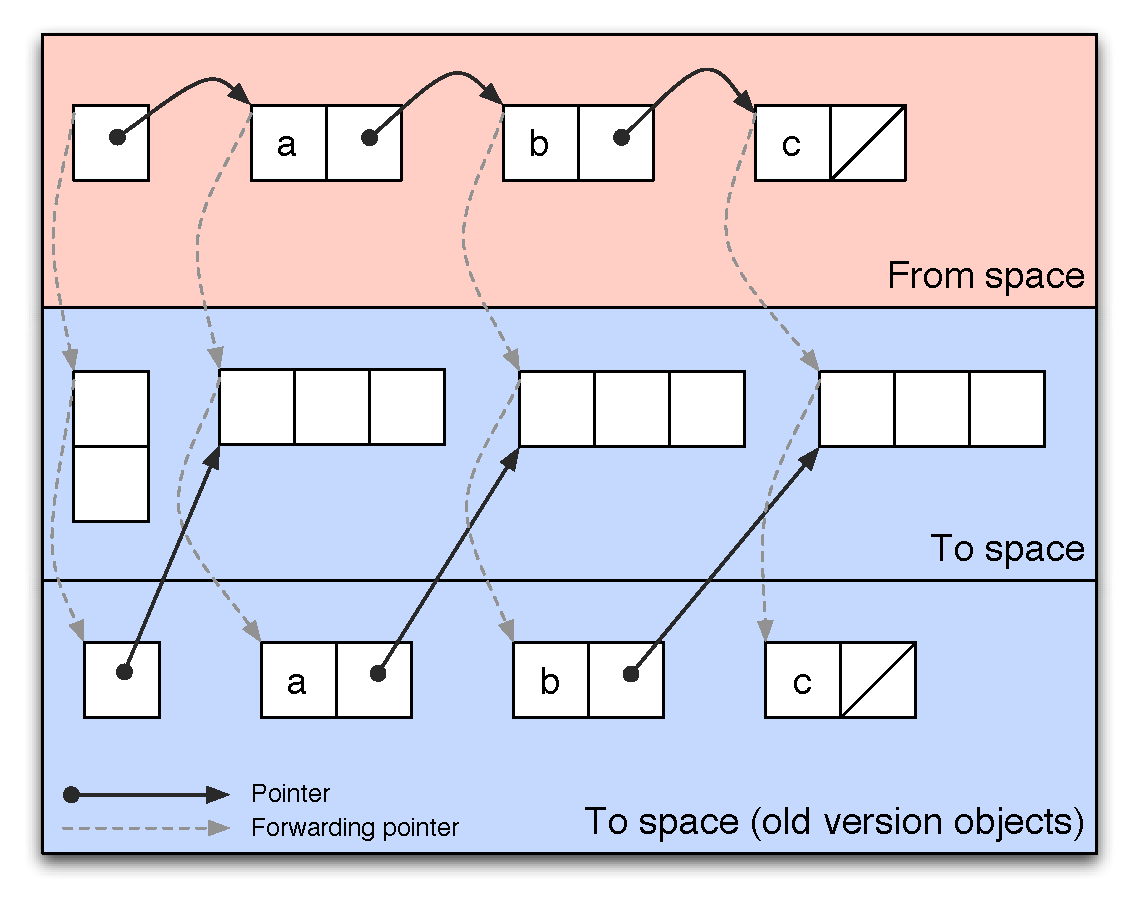
\includegraphics[scale=0.45]{images/singly-doubly/singly-doubly}}%
\end{column}
\begin{column}{0.3\paperwidth}
\begin{tiny}
\begin{verbatim}
jvolveObject(Node to, old_Node from) {
  to.data = from.data;
  to.next = from.next;
  if (to.next != null) {
    to.next.prev = to;
  }
}
\end{verbatim}
\end{tiny}
\end{column}
\end{columns}
\end{frame}

% \begin{frame}[t,fragile]{\DSU{} Garbage collector}%{A Sub-title is optional}
% \begin{itemize}
% \item Identical to Semispace for ``regular'' objects
% \item For objects to be transformed
%   \begin{itemize}
%   \item Copy the object to ToSpace (like Semispace)
%   \item Also, allocate an empty object in ToSpace for the new version
%   \end{itemize}
% \item Forwarding pointers point to the ``new version'' object
% \item No field can point to an ``old version'' object
% \end{itemize}
% \end{frame}

\ifdraft{}{
% 
%%%%%%%%%%%%%%%%%%%%%%%%%%%%%%%%%%%%%%%%%%%%%%%%%%%%%%%%%%%%%%%%%%%%%%%%
% Now, we show semispace with objects being updated.
%%%%%%%%%%%%%%%%%%%%%%%%%%%%%%%%%%%%%%%%%%%%%%%%%%%%%%%%%%%%%%%%%%%%%%%%
{
\begin{frame}[fragile]{\DSU{} garbage collector}%{A Sub-title is optional}
\setbeamercovered{invisible}
\begin{columns}[t]
\begin{column}[T]{0.67\paperwidth}
\begin{tikzpicture}
\begin{scope}
  % objects
  \uncover<1>{       \node[field] (root) at \objectRoot {root};                        }
  \uncover<2->{      \node[new space black field] (root) at \objectRoot {root};        }
                     \oldSpaceObject{A}{\objectA}
                     \oldSpaceObject{B}{\objectB}
                     \oldSpaceObject[dsu v0 object]{C}{\objectC}
                     \oldSpaceObject{D}{\objectD}
                     \oldSpaceObject{E}{\objectE}
                     \oldSpaceObject[dsu v0 object]{F}{\objectF}
                     \oldSpaceObject{G}{\objectG}
  % forwarding pointers
  \uncover<2->{      \forwardingPointer{A}                             }
  \uncover<3->{      \forwardingPointer{B}
                     \dsuForwardingPointer{C}                          }
  \uncover<4->{      \forwardingPointer{D}
                     \forwardingPointer{E}                             }
  \uncover<5->{      \dsuForwardingPointer{F}
                     \forwardingPointer{G}                             }
  % pointer arrows
  \uncover<1>   {    \path[regular]     (root.east)  to [out=330,in=120] (A.140)    ;          }
  \uncover<1>   {    \path[regular]     (A 0.center) to                (B.90)     ;            }
  \uncover<1>   {    \path[regular]     (A 1.center) to                (C.135)    ;            }
  \uncover<1-2> {    \path[regular]     (B 0.center) to                (D.135)    ;            }
  \uncover<1-2> {    \path[regular]     (B 1.center) to                (E.90)     ;            }
  \uncover<1-2> {    \path[regular]     (C 0.center) to                (F.135)    ;            }
  \uncover<1-2> {    \path[regular]     (C 1.center) to                (G.90)     ;            }
  \uncover<1-4> {    \path[regular]     (F 0.center) to                (A)        ;            }
                                                                      
  \uncover<2> {    \path[transparent]   (root.east)  to [out=0,in=120] (A.140)    ;            }
  \uncover<2> {    \path[transparent]   (A 0.center) to                (B.90)     ;            }
  \uncover<2> {    \path[transparent]   (A 1.center) to                (C.135)    ;            }
  \uncover<3> {    \path[transparent]   (B 0.center) to                (D.135)    ;            }
  \uncover<3> {    \path[transparent]   (B 1.center) to                (E.90)     ;            }
  \uncover<3> {    \path[transparent]   (C 0.center) to                (F.135)    ;            }
  \uncover<3> {    \path[transparent]   (C 1.center) to                (G.90)     ;            }
  \uncover<5> {    \path[transparent]   (F 0.center) to                (A)        ;            }

  \draw[draw,thin] (-4,-2.5) rectangle (4,0.5);
  \draw (4,0.5) node[anchor=north east,inner sep=1pt,font=\tiny] {FromSpace};

\end{scope}
\begin{scope}[yshift=-3.75cm]
  % objects
  \uncover<2>   {    \newSpaceGreyObject{A'}{\objectAprime}                          }
  \uncover<3->  {    \newSpaceBlackObject{A'}{\objectAprime}                         }

  \uncover<3>   {    \newSpaceGreyObject{B'}{\objectBprime}                          }
  \uncover<4->  {    \newSpaceBlackObject{B'}{\objectBprime}                         }

  \uncover<3-4> {    \dsuNewSpaceGreyObject{C'}{\objectCprime}                       }
  \uncover<5-10>{    \dsuNewSpaceBlackObject{C'}{\objectCprime}                      }
  \uncover<3->  {    \newSpaceVersionOneEmptyObject{C'}{\objectCprimeVersionOne}     }

  \uncover<4-5> {    \newSpaceGreyObject{D'}{\objectDprime}                          }
  \uncover<6->  {    \newSpaceBlackObject{D'}{\objectDprime}                         }

  \uncover<4-6> {    \newSpaceGreyObject{E'}{\objectEprime}                          }
  \uncover<7->  {    \newSpaceBlackObject{E'}{\objectEprime}                         }

  \uncover<5-7> {    \dsuNewSpaceGreyObject{F'}{\objectFprime}                       }
  \uncover<8-10>{    \dsuNewSpaceBlackObject{F'}{\objectFprime}                      }
  \uncover<5->  {    \newSpaceVersionOneEmptyObject{F'}{\objectFprimeVersionOne}     }

  \uncover<5-8> {    \newSpaceGreyObject{G'}{\objectGprime}                          }
  \uncover<9->  {    \newSpaceBlackObject{G'}{\objectGprime}                         }

  % pointer arrows
  \uncover<2->  {    \path[regular] (root.west)   to [out=220,in=95] (A'.north west);    }
  \uncover<2>   {    \path[regular] (A' 0.center) to [out=130,in=180] (B.west);
                     \path[regular] (A' 1.center) to [out=70,in=180]  (C.west);           }
  \uncover<3->  {    \path[regular] (A' 0.center) to [out=80,in=135]  (B'.150);          
                     \path[regular] (A' 1.center) to [out=270,in=110] (C' v1.north west); }
                                                                                         
  \uncover<3>   {    \path[regular] (B' 0.center) to                  (D.south);         
                     \path[regular] (B' 1.center) to                  (E.south);          }
  \uncover<4->  {    \path[regular] (B' 0.center) to [out=300,in=240] (D'.215);          
                     \path[regular] (B' 1.center) to [out=330,in=240] (E'.215);           }
                                                                                         
  \uncover<3-4> {    \path[regular] (C' 0.center) to                  (F.south);         
                     \path[regular] (C' 1.center) to                  (G.south west);     }
  \uncover<5-10>{    \path[regular] (C' 0.center) to [out=255,in=105]  (F' v1.north west);          
                     \path[regular] (C' 1.center) to [out=70,in=150]  (G'.150);           }
                                                                                         
  \uncover<5-7> {    \path[regular] (F' 0.center) to [out=30,in=325]  (A);                }
  \uncover<8-10>{    \path[regular] (F' 0.center) to [out=215,in=330] (A'.215);           }

  % transparent arrows
  \uncover<3>   {    \path[transparent] (A' 0.center) to [out=130,in=180] (B.west);
                     \path[transparent] (A' 1.center) to [out=70,in=180]  (C.west);       }

  \uncover<4>   {    \path[transparent] (B' 0.center) to                  (D.south);
                     \path[transparent] (B' 1.center) to                  (E.south);      }

  \uncover<5>   {    \path[transparent] (C' 0.center) to                  (F.south);
                     \path[transparent] (C' 1.center) to                  (G.south west); }

  \uncover<8>   {    \path[transparent] (F' 0.center) to [out=30,in=325]  (A);            }

  % v1 arrows
  \uncover<10-> {    \path[regular] (C' v1 0.center) to [out=30,in=120]   (F' v1.north west);
                     \path[regular] (C' v1 1.center) to                   (G'.210);          
                     \path[regular] (F' v1 0.center) to [out=180,in=315]  (A'.215);
                }
  

  \draw[draw,thin] (-4,-2) rectangle (4,0.5);
  \draw (4,-2) node[anchor=south east,inner sep=1pt,font=\tiny] {ToSpace};
\end{scope}
\end{tikzpicture}
\end{column}
\begin{column}[T]{0.25\paperwidth}
\begin{block}{}
\begin{tikzpicture}
\tikzstyle{column 2}=[anchor=west]
\matrix [row sep=0.5ex] {
\node[dsu v0 field] {};          & \node {\tiny To be transformed}; \\
\node[dsu v1 empty field] {};    & \node {\tiny $v_1$ object}; \\
};
\end{tikzpicture}
\end{block}

\begin{block}{}
\begin{footnotesize}
\only<1>{
The same heap as before. Objects to be transformed are highlighted.
}
\only<2>{
Copy A.
}
\only<3>{
Scan A'. Copy B and C. In addition an empty object C'$v_1$ is allocated.
\alert{A' points to this copy and not the old one.}
}
\only<4>{
Scan B'.
}
\only<5>{
Scan C'.
}
\only<6>{
Scan D'.
}
\only<7>{
Scan E'.
}
\only<8>{
Scan F'.
}
\only<9>{
GC is now complete. No field can point to C'$v_0$ or F'$v_0$. Pointers to C and
F point to $v_1$ (empty) objects. \texttt{memcpy(v\_1, v\_0);} will give us a valid
heap.}
\only<10>{
Setting fields of C'$v_1$ and F'$v_1$.
}
\only<11>{
C'$v_0$ and F'$v_0$ can be reclaimed.
}
\end{footnotesize}
\end{block}
\end{column}
\end{columns}
\end{frame}
}

% vim:tw=0:nospell

{
\begin{frame}[fragile]{\DSU{} Garbage collector}%{A Sub-title is optional}
\setbeamercovered{invisible}
\begin{center}
\begin{tikzpicture}
  % objects
                  \node[field] (root) at \objectRoot {root};
                  \oldSpaceObject{A}{\objectA}
                  \oldSpaceObject{B}{\objectB}
\uncover<-2>{     \dsuOldSpaceVersionZeroObject{C}{\objectC}                  }
                  \oldSpaceObject{D}{\objectD}
                  \oldSpaceObject{E}{\objectE}
\uncover<-2>{     \dsuOldSpaceVersionZeroObject{F}{\objectF}                  }
                  \oldSpaceObject{G}{\objectG}

                  \dsuOldSpaceVersionOneObject{C}{\objectCVersionOne}
                  \dsuOldSpaceVersionOneObject{F}{\objectFVersionOne}

                  % pointer arrows
                  \path[regular]     (root.east)  to [out=330,in=120]     (A.140);
                  \path[regular]     (A 0.center) to                      (B.90);
                  \path[regular]     (A 1.center) to                      (C v1.190);
                  \path[regular]     (B 0.center) to                      (D.135);
                  \path[regular]     (B 1.center) to                      (E.90);
\uncover<-2>{     \path[regular]     (C 0.center) to [out=180,in=90]      (F v1.north west);
                  \path[regular]     (C 1.center) to                      (G.90);
                  \path[regular]     (F 0.center) to                      (A);                       }

\uncover<2-3>{    \path[regular]     (C v1 0.center) to [out=180,in=120]  (F v1.north west);
                  \path[regular]     (C v1 1.center) to                   (G.60);
                  \path[regular]     (F v1 0.center) to                   (A);                       }

  \draw[draw,thin] (-4,-3.5) rectangle (4,0.5);
\end{tikzpicture}
% \begin{block}{}
% Loren ipsum. Hello World. Hello World. Hello World.  Loren ipsum. Hello World.
% Hello World. Hello World.  Loren ipsum. Hello World. Hello World. Hello World.
% Loren ipsum. Hello World.\footnote{This is a footnote} Hello World. Hello World.  Loren ipsum. Hello World.
% Hello World. Hello World.
% \end{block}
\end{center}
\end{frame}
}

% vim:tw=0:nospell

% {
\begin{frame}[fragile]{Revisiting transformation functions}%{A Sub-title is optional}
\setbeamercovered{invisible}
\begin{center}
\begin{tikzpicture}
  % objects
  \node[field] (root) at \objectRoot {root};
  \oldSpaceObject{A}{\objectA}
  \oldSpaceObject{B}{\objectB}
  \dsuOldSpaceVersionZeroObject{C}{\objectC}
  \oldSpaceObject{D}{\objectD}
  \oldSpaceObject{E}{\objectE}
  \dsuOldSpaceVersionZeroObject{F}{\objectF}
  \oldSpaceObject{G}{\objectG}
  \dsuOldSpaceVersionOneObject{C}{\objectCVersionOne}
  \dsuOldSpaceVersionOneObject{F}{\objectFVersionOne}

  % pointer arrows
  \path[regular]     (root.east)  to [out=330,in=120]     (A.140);
  \path[regular]     (A 0.center) to                      (B.90);
  \path[regular]     (A 1.center) to                      (C v1.190);
  \path[regular]     (B 0.center) to                      (D.135);
  \path[regular]     (B 1.center) to                      (E.90);
  \path[regular]     (C 0.center) to [out=180,in=90]      (F v1.north west);
  \path[regular]     (C 1.center) to                      (G.90);
  \path[regular]     (F 0.center) to                      (A);

  \draw[draw,thin] (-4,-3.5) rectangle (4,0.5);
\end{tikzpicture}
\begin{block}{We have an ordering problem}
\texttt{(C $v_0$).field0.field0} might be uninitialized
\end{block}
\end{center}
\end{frame}
}

% vim:tw=0:nospell

}

% \begin{frame}[t,fragile]{Revisiting transformation functions}%{A Sub-title is optional}
% Solutions to the ordering problem \\
% \begin{itemize}
% \item Programmer can invoke a VM function that will transform objects on
% demand. Moves burden of safety to the programmer
% \uncover<2>{
% \item Insert read barrier code to perform this check when compiling the
% transformation function
% \item Perform some static analysis to determine an order to queue
% objects
% }
% \end{itemize}
% \end{frame}

% \begin{frame}[fragile]{Updating from a singly to doubly linked list}%{A Sub-title is optional}
% \begin{footnotesize}
% \begin{verbatim}
% public static void jvolveObject(LinkedList.Node to,
%                                 r0_LinkedList.Node from) {
%   to.next = from.next;
%   to.data = from.data;
%   if (to.next != null) to.next.prev = to;
% }
% 
% public static void jvolveObject(LinkedList to, r0_LinkedList from) {
%   Jvolve.transformReferences(from);
%   to.head = from.head;
%   LinkedList.Node n0 = null;
%   LinkedList.Node n1 = to.head;
%   while (n1 != null) {
%     n0 = n1;
%     n1 = n1.next;
%   }
%   to.tail = n0;
% }
% \end{verbatim}
% \end{footnotesize}
% \end{frame}
